\section{Implementation}\label{s:impl}
\begin{figure*}[t]
    \centering
    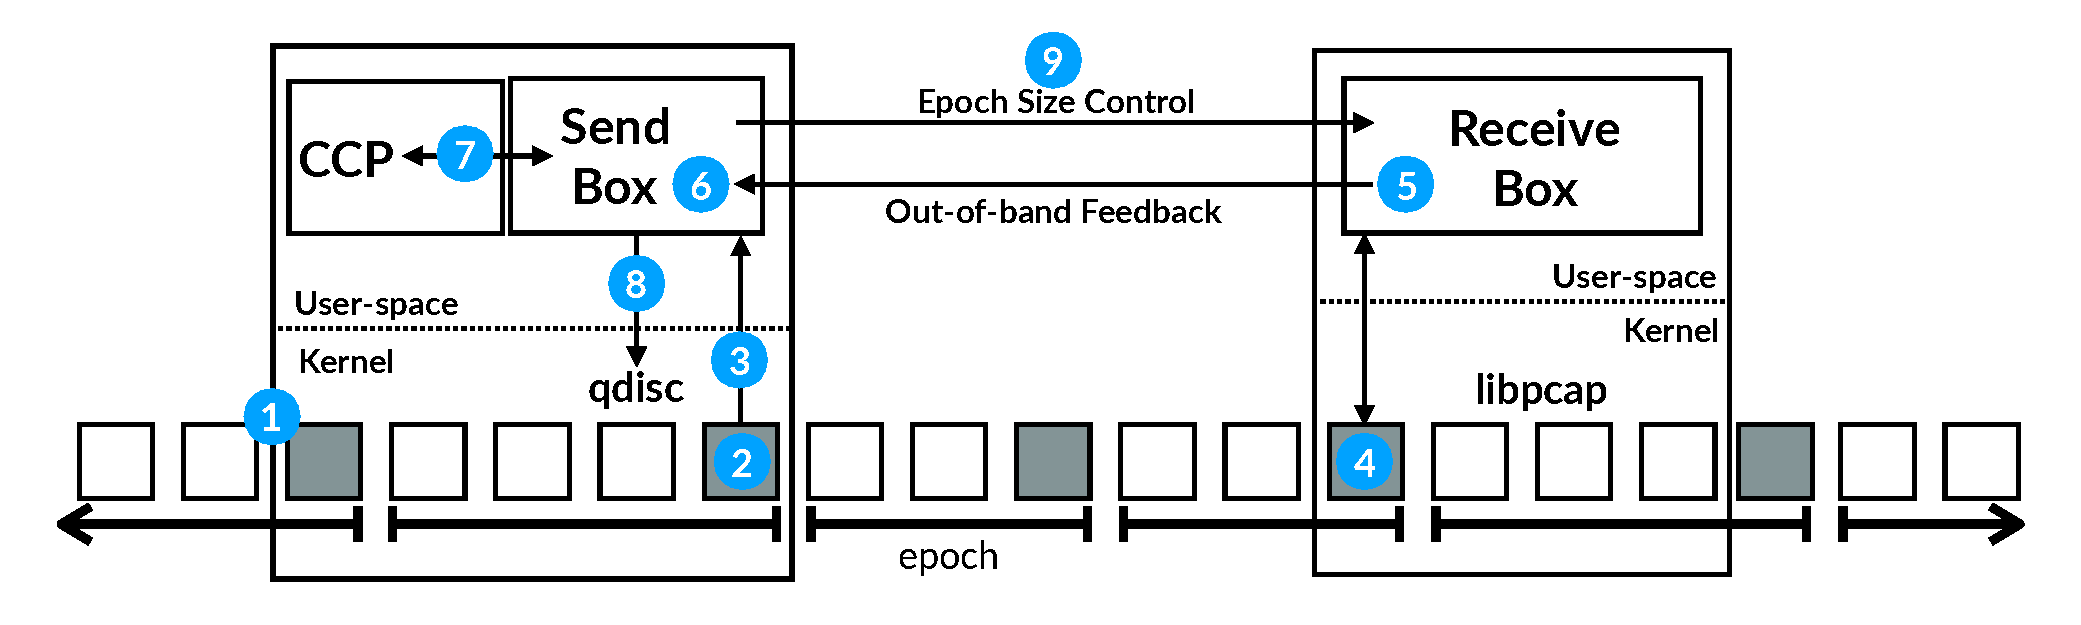
\includegraphics[width=2\columnwidth]{img/bundler-diagram}
    \caption{\name Implementation Overview.}\label{fig:bundler}
\end{figure*}

\cut{The prevalence of middleboxes today means that there are multiple options for implementing a \name \radhika{cut this line?}.}

\name boxes can be implemented as described below (although the specific implementations could vary across deployments).

\Para{\capinbox} It comprises of a \emph{data plane} and a \emph{control plane}. The data plane is responsible for (i) packet forwarding, (ii) tracking the number of sent bytes, (iii) identifying and reporting the epoch boundary packets to the control plane, (iv) enforcing a sending rate (computed by the control plane) on a bundle, and (iv) enforcing the desired scheduling policies for a bundle. It can implemented in software~\cite{bess, click, mos, netbricks, tc}, or in programmable hardware~\cite{p4}. The control plane, implemented in software, is responsible for (i) measuring congestion signals using the information provided by the data plane along with the feedback from the \outbox, (ii) computing and communicating epoch sizes, and (iii) running the congestion control algorithm for each bundle to compute appropriate sending rates based on the measured congestion signals. 

\Para{\capoutbox} It (i) tracks the number of received bytes, (ii) receives and updates epoch size values, (iii) identifies epoch boundary packets and sends feedback message to the \inbox up on receiving one. Similar to \inbox's data plane, it can also be implemented using either software or hardware.

% \vspace{0.05in}
% \noindent We next describe our prototype implementation (\ref{s:impl:prototype}) and illustrate how it works (\ref{s:impl:loop}). 

%\radhika{move to end, see comment at end of paragraph}.
% We describe a two-part design for the \inbox: a ``control plane'' and ``data plane'' separation.
% The data plane is responsible for packet forwarding, maintaining a count of the \cut{in-bundle} bytes sent, enforcing a rate and scheduling policy on the bundle, and reporting epoch boundary packets to the control plane.
% These operations can be implemented either in software, via modern platforms for network function virtualization~\cite{bess, click, mos, netbricks}, or in hardware via programmable switches~\cite{p4} \radhika{move to end, see comment at end of paragraph}.
% The control plane is responsible for computing measurements by combining feedback from the data plane and \outbox, and running the congestion control logic necessary to pick the appropriate rate for each bundle.
% The \outbox is simple and does not require a control plane; it simply must observe the packet stream, maintain a byte count, and send reports to the \inbox on observing epoch packets.
% The \outbox can, therefore, be implemented entirely in hardware if necessary \radhika{cut}.
% \radhika{We envision the control plane to be implemented in software, while the data plane can be implemented in...(the line you had before)}


\subsection{Prototype}\label{s:impl:prototype}

We now describe our prototype implementation of the \name boxes.

\Para{\capinbox data plane} We implement it using Linux \texttt{tc}~\cite{tc}.
%and we limit our scheduling policy to those available in the Linux kernel.
We patch the TBF queueing discipline (qdisc)~\cite{tbf} to detect epoch boundary packets, and to report them to the control plane using a netlink socket. We use the FNV hash function~\cite{fnv-hash}, a non-cryptographic fast hash function with a low collision rate, to compute the packet content hash for identifying epoch boundaries.
%, and make the internal scheduling policy configurable.
We patch TBF's ``inner\_qdisc'' to support SFQ~\cite{sfq}, FQ-CoDel~\cite{fq-codel} and strict prioritization, in addition to the default FIFO. 
By default, TBF instantaneously re-fills the token bucket when the rate is updated; we disable this feature to avoid rate fluctuations caused by our frequent rate updates. 
Our patches to the TBF qdisc comprise $112$ lines of C.
%\an{cut?}\an{Additionally, we remove one line in the rate update to disable re-filling the token bucket on rate changes to prevent a penalty for frequent rate updates\footnote{}.}

% For our prototype, we implement the \inbox data plane using Linux \texttt{tc}~\cite{tc}, and we limit our implementations of scheduling policy to those already widely available in the Linux kernel.
% We patch the TBF queueing discipline (qdisc)~\cite{tbf} to detect epoch boundary packets, transmit feedback to the control plane using a netlink socket, and make the internal scheduling policy configurable.
% We express scheduling policy by changing TBF's ``inner\_qdisc'' from the default FIFO to a work-conserving, scheduling qdisc: we support SFQ~\cite{sfq} and FQ-CoDel~\cite{fq-codel}.
% Our patch to the TBF qdisc comprises $112$ lines of C.
% \an{cut?}\an{Additionally, we remove one line in the rate update to disable re-filling the token bucket on rate changes to prevent a penalty for frequent rate updates\footnote{by default, TBF instantaneously re-fills the token bucket when the set rate changes. In our implementation, the \inbox sets the rate frequently, causing rate fluctuations. We therefore disable this functionality.}.}

\Para{\capinbox control plane} We implement it to run in user-space in $1167$ lines of Rust.
We use CCP~\cite{ccp} to run different congestion control algorithms (described next). CCP is a platform for expressing congestion control algorithms in an asynchronous format, which makes it a natural choice for our epoch-based measurement architecture. The control plane uses \texttt{libccp}~\cite{ccp} to interface with the congestion control algorithm, and  \texttt{libnl} to communicate with the qdisc.

\Para{Congestion control algorithms} We use existing implementations of congestion control algorithms (namely, Nimbus~\cite{nimbus}, Copa~\cite{copa} and BBR~\cite{bbr}) on CCP to compute sending rates at the \inbox.  If the algorithm uses a congestion window, the \inbox computes an effective rate of $\frac{\text{CWND}}{\text{RTT}}$ and set it at the qdisc. We validated that our implementation of these congestion control schemes at the \inbox closely follows their implementation at an endhost.
%endhost 
%to be the minimum of the explicit rate and this effective rate.
%Upon receiving new RTT samples, the \inbox updates the effective rate, and updates the qdisc rate if appropriate.

The \inbox also leverages a recently proposed technique~\cite{nimbus} to detect persistent buffer-filling flows. Its basic idea is to use short-timescale pulses to create traffic fluctuations at the bottleneck link, and measure if the cross traffic changes its rate in response to these fluctuations; if it does, it indicates the presence of long-running TCP flows that react to bandwidth variations. When such flows are detected, the \inbox  starts pushing traffic at an increased rate, set to the observed received rate plus a probe factor. Sending faster than the receive rate ensures that the rate of the \inbox eventually exceeds the offered load, thus draining any queue at the \inbox. This, in turn, allows the congestion control algorithms at the unmodified endhosts to compete with the buffer-filling flow, as they would without a \name. The additive probe factor is set in our implementation to one-sixteenth of the maximum receive rate seen so far. 

%It maintains the congestion control state of each bundle, but does not maintain (or observe) per-flow state.
%\radhika{no. of LoC for \inbox dataplane?} \an{first paragraph of this section?}

\Para{\capoutbox} We implement it using \texttt{libpcap} in $188$ lines of Rust. 
%It listens for packets on the interface, checks for epoch packets, and sends the reports to the \inbox. It must maintain per-bundle counters (described in \S\ref{s:impl:discovery}).

\subsection{\name Event Loop}\label{s:impl:loop}
Figure~\ref{fig:bundler} provides an overview of how our \name implementation operates.

(1) Packets arriving at the \inbox are sent to the qdisc. Those that match a bundle are put into the proper queue, 
otherwise they are forwarded immediately. (2) The qdisc determines whether a packet matches the epoch boundary
condition (\S\ref{s:measure:marking}). (3) If so, it sends a netlink message to the control plane process running in user-space, and then forwards the packet along. The control plane process records the epoch boundary packet (\S\ref{s:measure:compute}) (4) The \outbox observes the same epoch boundary packet. (5) It sends an out-of-band UDP message to the \reword{\inbox} that contains the hash of the packet and its current state. (6) The \reword{\inbox} receives the UDP message, and uses it to calculate the epochs and measurements as described 
in \S\ref{s:measurement}. 
(7) Asynchronously, the \inbox control plane invokes the congestion control algorithm every $10$ms~\cite{ccp}
%\footnote{Prior work shows~\cite{ccp} that the datapath need only invoke congestion control algorithms on RTT-timescales, and evaluates congestion control algorithms on their sensitivity to this period.}.
via \texttt{libccp},
%giving it a chance to observe any new measurements and change its behavior. 
(8) The \inbox control plane communicates the rate, if updated, to the qdisc
using \texttt{libnl}. 
% Since the qdisc only supports rate enforcement, if the algorithm
% also uses a congestion window, the \inbox computes $\text{\emph{effective rate}} = \frac{\text{CWND}}{\text{RTT}}$
% and sets the rate of the qdisc to the minimum of the explicit rate and this effective rate.
%Upon receiving new RTT samples, the \inbox updates the effective rate, and updates the qdisc rate if appropriate.
Finally (9), if the \inbox changes the desired epoch length based on new measurements, it communicates this to the \outbox, also out-of-band.

%\radhika{i liked this subsection!}





%\radhika{an experiment showing scalability of bundler implementation?}

%\subsection{Congestion Control}\label{s:impl:cc}
%We use existing implementations of congestion control algorithms on CCP~\cite{ccp}, a platform for expressing congestion control algorithms in an asynchronous format; since CCP algorithms are already designed to receive network feedback asynchronously, they are a natural choice for our epoch-based measurement architecture. \radhika{this sentence should comer earlier, maybe when you first mention ``control-plane'' at the beginning of Sec 5, especially since 5.2 mentions CCP and libccp.}

%\an{move to earlier, maybe design:}
%It is important to note that traditional loss-based congestion controllers (\ie Cubic~\cite{cubic}, NewReno~\cite{newreno}) are poor choices for \name. 
%This is because they double-penalize component traffic for losses: first, in the reaction of the end-to-end congestion controller to the loss, and second in the reaction of the controller at \name.

%\an{missing connection here}
%Therefore, for algorithms which observe loss (Nimbus and Copa), we configure them to ignore it; the end-to-end reaction to loss will modulate the offered load to be the fair share of the bottleneck.
%
%Further, we make a useful distinction between two types of cross-traffic conditions \name will experience.
%We consider \emph{elastic} cross traffic and \emph{inelastic} cross traffic.
%Elastic cross traffic (\eg Cubic, NewReno) probes for bandwidth and fills buffers at the bottleneck; inelastic cross traffic (\eg short flows) has limited demand and does not fill buffers.

%When cross traffic is inelastic, the queueing delays that \name encounters will be self-inflicted. In these scenarios, scaling back and adjusting the sending rate at \inbox will cause the bottleneck to shift and the queueing delays at the bottleneck to reduce.
%In the presence of elastic cross traffic, however, congestion control algorithms \emph{must} push packets into the bottleneck queue to remain competitive~\cite{bbr, copa, nimbus}.
%As a result, we expect \name's benefits to disappear, since it must relinquish control of the queues to the bottleneck link.

%\radhika{if above parts are covered in Sec 3, add a backwards pointer, and start with the implementation details below.}

% Recent work~\cite{copa, nimbus} has considered the problem of switching between modes to take advantage of low queueing delays when it is possible to do so, yet reacting to and competing fairly with elastic cross traffic when it present.
% Unfortunately, it is not immediately clear how to determine \name's fair rate once we detect elastic cross traffic.
% The number of individual component connections which are backlogged at any given time may vary, and determining which connections should count towards \name's aggregate fair share rate would thus require per-connection state \radhika{not super clear to me}.

% We sidestep this issue with a simple, yet powerful, observation: rather than attempt to compete with elastic cross traffic, \name should \emph{get out of the way} of its component connections.
% The end-to-end congestion controllers responsible for \name's component connections will then naturally compete with and achieve their fair rate against elastic cross traffic.

% It is important to implement this approach carefully. 
% Consider a naive implementation in which upon detecting elastic cross traffic, \name stopped pacing packets entirely.
% This approach would be unable to detect when the elastic cross traffic subsided, since it yields all control over the network queues.

% Thus, when \name's congestion control algorithm detects that the cross traffic is elastic, it uses a simple control rule: \texttt{rate <- observed\_receive\_rate * 1.25}. 
% This control rule will rapidly grow the pacing rate at the \inbox until it stabilizes at 25\% above the offered load.
% Then, using the elasticity detection mechanism described in prior work~\cite{nimbus}, \inbox can modulate the pacing rate to determine when to retake control of the queueing, and therefore the scheduling policy.

% \an{move the elastic cross traffic comparison results here?} \radhika{no, add a forward pointer}
